\documentclass[a4paper, 12pt]{article}
\usepackage[T1]{fontenc}
\usepackage[utf8]{inputenc}
\usepackage{apacite}
\usepackage{mathptmx}
\usepackage{enumerate}
\usepackage[margin=0.5in]{geometry}
\usepackage{xspace}
\usepackage{graphicx}
\usepackage{tikz}
\usepackage{makecell}
\usetikzlibrary{shapes.geometric, arrows.meta}
\usepackage{multirow}
\usepackage[table]{xcolor}
\usepackage{float}

\renewcommand{\baselinestretch}{1.0}

\newcommand\nd{\textsuperscript{nd}\xspace}
\newcommand\rd{\textsuperscript{rd}\xspace}
\newcommand\nth{\textsuperscript{th}\xspace} %\th is taken already

% Increase the space between paragraphs
\setlength{\parskip}{1em}
\setlength\parindent{0pt} % set paragraph indent to zero

% fill up your name, ID, contribution and paper title here
\author{
Lai Leong Chun \quad 241UC240JR \quad 34\% \\
Teh Li Wei \quad 1211109581 \quad 33\%\\
Sow Chien Yee \quad 1211210800 \quad 33\%\\
}
\title{ Research Proposal on Anti-Cheating Methods in Competitive Games  }

\begin{document}
\maketitle

\section*{Executive Summary}
This research proposal tackles the urgent problem of cheating in competitive gaming, especially within the rapidly growing esports sector, where maintaining integrity is crucial. Despite progress in anti-cheat technologies, current solutions often falter in adapting to new cheating methods and lack generalized, scalable frameworks suitable for various game genres and platforms. This proposal seeks to investigate hybrid detection methods that fuse kernel-level techniques with adaptive detection mechanisms, thereby addressing notable gaps in existing literature, including adaptability limitations, real-time detection efficacy, and data privacy issues. The primary objectives are to develop a robust anti-cheat system designed to enhance detection accuracy, minimize false positives, and create a cross-platform framework that guarantees fairness and security in competitive gaming. Ultimately, the aim is to uphold the competitive integrity of esports while fostering player trust and ensuring compliance with data protection regulations.
\hfill
\\
\textbf{Keywords:} anti-cheat systems, competitive gaming, machine learning, cheating detection, esports integrity \\
\newpage
\tableofcontents
\newpage
\section{Introduction}
The focus of this research proposal is on anti-cheating methods in competitive gaming, with a particular emphasis on First-Person Shooter (FPS) games and various competitive online platforms. As esports emerges as a multi-billion dollar industry, maintaining fair play is essential to uphold the integrity of gaming competitions. Cheating—ranging from visual hacks like aim-bots to more complex network manipulation—continues to undermine player trust and degrade the overall gaming experience. While several strategies have been proposed to combat cheating, including kernel-level solutions that operate at a low system level to detect unauthorized modifications, existing approaches often struggle to keep pace with the rapidly evolving landscape of cheating techniques and lack scalability across diverse gaming environments. This proposal seeks to address these limitations by investigating advanced kernel-level detection methods that ensure robust security and integrity in competitive gaming.

\section{Problem Statement}
Cheating in competitive games remains a significant challenge despite advances in anti-cheat technologies. Existing solutions often fail to scale in real-time gaming environments and are limited in their ability to adapt to new cheating techniques, leading to persistent exploitation and frustration among players. There is also a lack of generalized solutions that can be applied across different gaming platforms, leaving room for more holistic approaches.

\subsection{Research Gaps}
\begin{itemize}
    \item \textbf{Lack of Holistic Solutions}: The existing literature often focuses on specific cheating methods, such as visual hacks or game bots, and lacks approaches that can effectively address a broader range of cheating practices, including network manipulation, server-side exploits, or more nuanced forms of cheating like exploiting game mechanics or match-fixing.
    \item \textbf{Limited Cross-Platform Focus}: The majority of studies concentrate on specific game genres, like first-person shooters or role-playing games, and offer limited insights into how anti-cheat mechanisms might be applied across different platforms (PC, mobile, console) or game types. Since cheating strategies can vary significantly across platforms, the absence of cross-platform research creates a notable gap in understanding.
    \item \textbf{Scalability and Real-Time Detection}: Some existing works focus on frame analysis, which presents difficulties in scaling for real-time environments that demand high traffic management and low latency. There is a pressing need for research that aims to improve detection systems for real-time use while maintaining accuracy, particularly within the esports context.
    \item \textbf{Data Privacy and Ethical Concerns}: Only a few studies address potential privacy issues that may arise from monitoring player behaviour and collecting large amounts of data for cheat detection. As anti-cheat technologies become increasingly invasive, it’s vital to focus more on data privacy issues, especially in mobile and online gaming, to maintain player trust and ensure compliance with regulations.
\end{itemize}

\subsection{Justification}
The economic and social stakes in esports are growing, with professional players and game developers investing millions in competitive events. Therefore, maintaining fairness is crucial. The development of a scalable and adaptable anti-cheating system will help preserve competitive integrity, protect the reputation of games, and prevent economic loss due to cheating-induced player attrition.

\section{Research Questions, Hypotheses and Objectives}
\subsection{Research Questions}
    \begin{enumerate}
        \item How can a hybrid anti-cheat system that integrates kernel-level techniques with adaptive detection mechanisms enhance the identification of cheating behaviors in competitive gaming environments?
        \item What are the primary limitations of existing anti-cheat technologies, and how can a generalized framework be developed to effectively combat cheating across various gaming genres and platforms?
    \end{enumerate}
\subsection{Research Hypotheses}
\begin{enumerate}
    \item Implementing a hybrid anti-cheat system that combines kernel-level detection with advanced adaptive mechanisms will significantly reduce false positives and improve the accuracy of detecting emerging cheating techniques.
    \item A generalized anti-cheat framework designed for cross-platform adaptability will enhance the scalability and flexibility of detection methods, resulting in fairer competitive gaming experiences across different platforms and genres.
\end{enumerate}
\subsection{Research Objectives}
\begin{enumerate}
    \item To design and develop a hybrid cheat detection system that employs kernel-level techniques alongside adaptive detection methods to improve precision and reduce error rates.
    \item To evaluate and optimize the scalability and real-time performance of the proposed anti-cheat system in high-stakes environments, such as esports tournaments, ensuring it meets the demands of low-latency gameplay.
    \item To establish a comprehensive and generalized cheat detection framework applicable across multiple gaming platforms (PC, console, mobile) and diverse genres (FPS, RPG, etc.), facilitating a unified approach to cheating prevention.
    \item To assess the effectiveness of the hybrid anti-cheat system in minimizing false positive rates and enhancing detection capabilities for new and evolving cheating strategies while ensuring compliance with data privacy regulations.
\end{enumerate}

\section{Literature Review}
The evolution of anti-cheating methods in FPS or competitive gaming has benefited significantly from the integration of artificial intelligence (AI) and machine learning technologies.  Recent research has explored various innovative approaches to detecting cheating behaviour, focussing primarily on vision-based detection \cite{zhao_2023_vespa}, trajectory analysis \cite{su_2022_fewshot} and behavioural-based detection \cite{cao_2024_beat}. These methods leverage deep learning models such as confidence analysis and IBP to enhance accuracy and adaptability in dynamic gaming environments.

Studies indicate that visual detection methods using deep neural networks (DNNs) \cite{jonnalagadda_2021_robust} and other machine learning algorithms have strong practical applications. By analysing frame buffers within games, these approaches can identify common visual cheats that are called ESP such as aim bots and wall hacks. This gives players access to information they would not normally have, such as the location of hidden opponents. This innovative detection strategy offers a more effective means of capturing and recognising the complexities of cheating compared to traditional input monitoring methods.

However, despite their promising performance, these methods face several challenges in the future. Many frameworks struggle with limited labelled data, especially as new cheating patterns continuously emerge and evolve at a fast pace. This necessitates that anti-cheat systems possess high adaptability, allowing them to adjust and update in response to evolving cheating strategies quickly. Furthermore, reliance on smaller sample sizes and specific games or cheat software limits the broader applicability of these studies. In addition, many systems rely on vision-based detection, which uses a large amount of computational resources, making it difficult to implement in real time, especially in environments with millions of active players.

Another critical issue is the scalability and false positive rates of these systems. While many models perform well in specific games, their effectiveness may vary when applied to different types or genres of games. False positives not only result in unfair bans, but also erode trust between players and game developers. For example, DNNs, though highly accurate in some scenarios, are computationally intensive and struggle to operate efficiently in real-time environments, particularly in large-scale settings like esports tournaments. Moreover, few-shot learning is limited in its ability to generalise well to new forms of cheating techniques, as it requires constant retraining and updating to keep up with the rapidly evolving nature of cheating. The absence of human oversight in many systems exacerbates this issue, as there is no secondary layer of validation to ensure that flagged behaviour is genuinely suspicious. Thus, developing systems with automatic updating mechanisms and robust generalisation capabilities is vital for future research.

In summary, while current anti-cheat systems have made significant strides in reducing cheating in competitive games, they remain limited in terms of scalability, adaptability, and accuracy. They not only provide new detection methodologies, but also reveal the technological challenges of maintaining fair competition in an ever-changing cheating landscape. Ongoing research will be crucial in exploring more diverse and efficient anti-cheating solutions to ensure fairness and enhance player experience in competitive gaming.

\section{Research Methodology}
Rootkit anti-cheating software represents a significant advancement in the fight against cheating in online gaming. These systems operate at a deep system level, similar to rootkits, allowing them to detect and prevent a wide range of cheating methods. However, their potential to address the broader issues in anti-cheat solutions is particularly noteworthy. A critical analysis of kernel-level anti-cheat systems demonstrates that these systems offer robust cheat detection but introduce significant privacy risks, as they operate with deep access to system resources \cite{dorner_2024_if}.

Firstly, rootkit anti-cheating software can provide holistic solutions to cheating. Traditional anti-cheat methods often focus on specific types of cheating, such as visual hacks or game bots. In contrast, rootkit-based systems can tackle more diverse and complex forms of cheating, including network manipulation, server-side exploits, and subtle social engineering cheats like exploiting game mechanics or match-fixing. For example, FACEIT Anti-Cheat and Vanguard were found to utilise techniques that start at boot up to ensure a trusted system state, monitoring drivers and threads from the kernel level, thus preventing tampering \cite{dorner_2024_if}. This broad monitoring allows these systems to detect sophisticated cheating tactics that standard anti-cheat measures might miss.

Secondly, these systems have the potential to address the limited cross-platform focus seen in many anti-cheat solutions. Most of the literature and solutions exist that are tailored to specific genres or platforms of games, such as FPS or RPGs, and often neglect the differences in cheating tactics across platforms such as PC, mobile and console. Rootkit anti-cheating software, with its deep system integration, can be adapted to various platforms, providing a more unified and comprehensive approach to cheating prevention across different gaming environments. For example, both BattlEye and Easy Anti-Cheat have demonstrated adaptability to various platforms, ensuring that these solutions can provide a consistent level of security across multiple game titles \cite{dorner_2024_if}.

Thirdly, rootkit anti-cheating software can enhance scalability and real-time detection capabilities. Traditional methods, such as frame analysis, struggle to scale in real-time environments with high traffic and low latency requirements, especially in esports. Rootkit-based systems, however, can be optimized for real-time application without compromising accuracy. Their deep integration allows for more efficient monitoring and quicker response times, making them suitable for the fast-paced nature of competitive gaming. FACEIT Anti-Cheat and Vanguard, both based heavily on kernel-level monitoring, exemplify how these systems can operate in real time, providing faster responses to cheats while keeping the integrity of the game intact \cite{dorner_2024_if}.

\begin{table}[H]
    \centering
    \resizebox{\textwidth}{!}{
    \begin{tabular}{lcccccccc}
        \makecell{\textbf{System}} & \makecell{\textbf{Evasion}} & \makecell{\textbf{Virtualization}} & \makecell{\textbf{Time of} \\ \textbf{Execution}} & \makecell{\textbf{Remote} \\ \textbf{Access}} & \makecell{\textbf{Information} \\ \textbf{Exfiltration}} & \makecell{\textbf{Network} \\ \textbf{Manipulation}} & \makecell{\textbf{Removability}} & \makecell{\textbf{Sum}} \\
        \hline
        BattlEye & $\circ$ & $\bullet$ & $\circ$ & $\bullet$ & $\bullet$ & $\circ$ & $\circ$ & 3 \\
        Easy Anti-Cheat & $\circ$ & $\bullet$ & $\circ$ & $\circ$ & $\bullet$ & $\circ$ & $\circ$ & 2 \\
        FACEIT Anti-Cheat & $\bullet$ & $\bullet$ & $\bullet$ & $\circ$ & $\bullet$ & $\circ$ & $\bullet$ & 5 \\
        Vanguard & $\bullet$ & $\bullet$ & $\bullet$ & $\circ$ & $\bullet$ & $\circ$ & $\circ$ & 4 \\
        Flame & $\bullet$ & $\circ$ & $\circ$ & $\bullet$ & $\bullet$ & $\bullet$ & $\bullet$ & 5 \\
    \end{tabular}
    }
    \caption{Overview of the analysed anti-cheat systems, including a comparison with the Flame rootkit.}
    \label{tab:anti_cheat_comparison}
\end{table}

A new anti-cheat solution should integrate the advanced evasion and virtualisation techniques of Vanguard, the early execution capability of both FACEIT and Vanguard, controlled remote access for adaptability, thorough information collection for detection, and improved network manipulation detection. Additionally, transparent and secure removability is crucial to ensuring user trust and system integrity. Combining these features will result in a robust, effective, and user-friendly anti-cheat solution \cite{dorner_2024_if}.

Despite these advantages, rootkit anti-cheating software shares some common weaknesses. These include potential privacy concerns, as they operate at a deep system level and can access sensitive information. The study highlights that systems such as Vanguard and FACEIT Anti-Cheat, which require the system to boot in a trusted state and monitor processes from start-up, present privacy risks that mimic the behaviour of rootkits \cite{dorner_2024_if}. In addition, its intrusive nature can lead to system instability and conflicts with other software. To address these issues, developers must prioritise transparency and user consent, ensuring that players are aware of and agree to the level of access these systems require. Furthermore, continuous updates and collaboration with cybersecurity experts can help mitigate risks and improve the reliability of these solutions \cite{dorner_2024_if}.

A promising alternative to mitigating privacy concerns is to harness the power of AI for handling anti-cheating tasks. By delegating the detection and prevention of cheating entirely to AI, we could ensure that no human operators have direct access to sensitive user data. AI systems, unlike human moderators, would have no incentive to exploit or misuse private information, as they would only process data according to their programmed objectives. However, it is crucial to establish strict limitations on AI's access and operations, ensuring that AI systems are granted only the minimal necessary permissions to perform their tasks effectively. By regulating AI’s control over sensitive information and incorporating ethical safeguards, we can reduce the risks associated with deep system monitoring without sacrificing efficiency. This approach would add another layer of privacy protection, as AI would serve as an impartial entity that could manage cheat detection autonomously while minimizing human interference in private data.

Moreover, to develop an anti-cheating system that is near perfect, we should aim to combine all the strengths of existing anti-cheat software. A comprehensive system could incorporate deep system-level monitoring of rootkit-based methods for robust cheat detection, the cross-platform adaptability of solutions like BattlEye and Easy Anti-Cheat, and the scalability and real-time responsiveness seen in FACEIT Anti-Cheat and Vanguard. By integrating these strengths, alongside AI-driven privacy protections, such a system could provide a highly effective, secure, and ethical solution to cheating. This unified approach could create an anti-cheat system that not only addresses existing weaknesses but also stands as a nearly flawless software, ensuring both gaming fairness and user privacy protection.

In conclusion, while rootkit anti-cheating software offers promising solutions to many of the current challenges in anti-cheat technology, it is crucial to address their inherent weaknesses through careful design and ethical considerations. In doing so, these systems can provide robust and comprehensive protection against cheating, enhancing the integrity and fairness of online gaming. The integration of AI into these systems offers a further safeguard by removing human operators from sensitive data access, thus mitigating privacy risks. By combining the best features of existing anti-cheat technologies and AI safeguards, the future of anti-cheat software could move toward a near-perfect solution, one that balances both robust cheat detection and the protection of user rights.

\section{Research Activities and Milestones}

\begin{figure}[H]
    \centering
    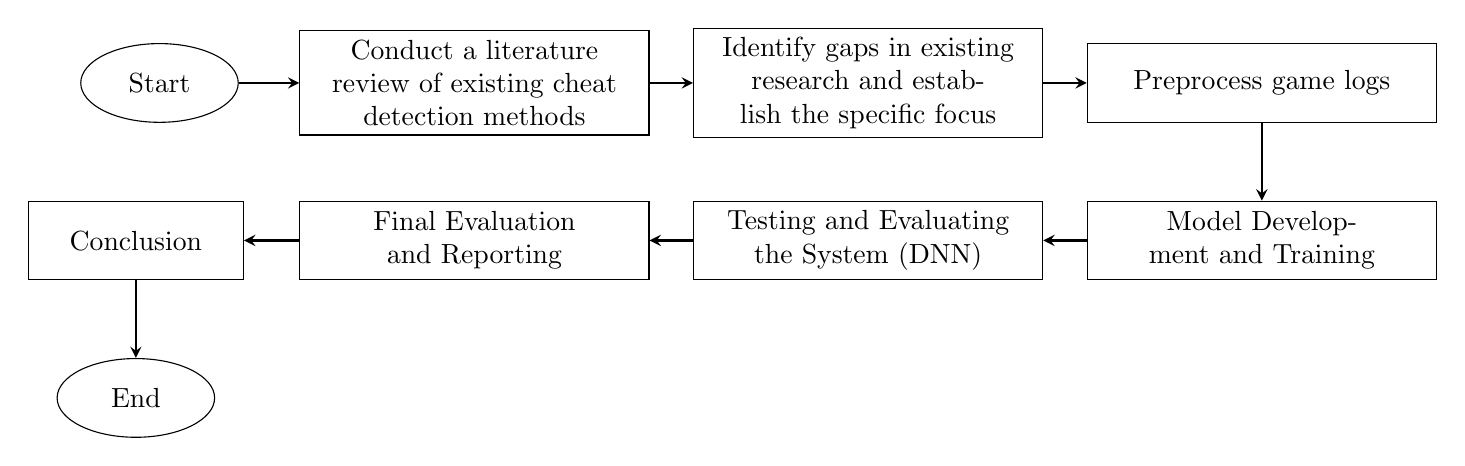
\begin{tikzpicture}[node distance=2cm, >=Stealth, auto]
    
    \tikzstyle{startstop} = [ellipse, minimum width=2cm, minimum height=1cm,text centered, draw=black]
    \tikzstyle{process} = [rectangle, minimum width=3cm, minimum height=1cm, text centered, draw=black, text width=4.2cm]
    \tikzstyle{arrow} = [thick,->,>=stealth]
    
    % Nodes
    \node (start) [startstop] {Start};
    \node (process1) [process, right of=start, xshift=2cm] {Conduct a literature review of existing cheat detection methods};
    \node (process2) [process, right of=process1, xshift=3cm] {Identify gaps in existing research and establish the specific focus};
    \node (process3) [process, right of=process2, xshift=3cm] {Preprocess game logs};
    \node (process4) [process, below of=process3] {Model Development and Training};
    \node (process5) [process, left of=process4, xshift=-3cm] {Testing and Evaluating the System (DNN)};
    \node (process6) [process, left of=process5, xshift=-3cm] {Final Evaluation and Reporting};
    \node (process7) [process, left of=process6, xshift=-2.3cm, minimum width=2.5cm, text width=2.5cm] {Conclusion};
    \node (stop) [startstop, below of=process7] {End};
    
    % Arrows
    \draw [arrow] (start) -- (process1);
    \draw [arrow] (process1) -- (process2);
    \draw [arrow] (process2) -- (process3);
    \draw [arrow] (process3) -- (process4);
    \draw [arrow] (process4) -- (process5);
    \draw [arrow] (process5) -- (process6);
    \draw [arrow] (process6) -- (process7);
    \draw [arrow] (process7) -- (stop);
    
    \end{tikzpicture}
    \caption{A flowchart illustrating the research activities.}
    \label{fig:flowchart_research_activities}
\end{figure}

\begin{table}[H]
    \centering
    \begin{tabular}{|m{7cm}|m{5cm}|c|c|}
        \hline
        \textbf{Activities} & \textbf{Milestones} & \textbf{Start Date} & \textbf{End Date} \\ \hline
        Conduct a literature review of existing cheat detection methods & \multirow{2}{*}{\parbox{5cm}{Completion of the literature review and problem definition}} & 8/9/2023 & 12/10/2023 \\ \cline{1-1} \cline{3-4}
        Identify gaps in existing research and establish the specific focus & & 30/10/2023 & 26/11/2023 \\ \hline
        Collect and curate datasets for both visual and behavioural cheat detection & \multirow{2}{*}{\parbox{5cm}{Completion of dataset collection and preprocessing}} & 4/12/2023 & 29/1/2024 \\ \cline{1-1} \cline{3-4}
        Preprocess game logs &  & 2/2/2024 & 24/2/2024 \\ \hline
        Model Development and Training & Models Developed and Trained (vision-based model and behavioural-based) & 5/3/2024 & 29/5/2024 \\ \hline
        Testing and Evaluation the system (DNN) & System Tested, Models Fine-tuned & 1/6/2024 & 23/8/2024 \\ \hline
        Final Evaluation and Reporting & Final System Evaluation, Report and Presentation Submitted & 31/8/2024 & 25/9/2024 \\ \hline
    \end{tabular}
    \caption{Research Activities and Milestone}
    \label{tab:research_activities}
\end{table}

\begin{table}[H]
    \centering
    \resizebox{\textwidth}{!}{
    \begin{tabular}{|m{3.7cm}|m{0.7cm}|m{3.0cm}|m{0.7cm}|m{3.0cm}|m{1.2cm}|m{3.0cm}|m{1.0cm}|m{2.5cm}|m{2.5cm}|}
        \hline
        \multirow{3}{*}{\parbox{4cm}{\textbf{Research Activities}}} & \multicolumn{9}{c|}{\textbf{Milestones}} \\ \cline{2-10}
        & \multicolumn{3}{c|}{\textbf{2023}} & \multicolumn{6}{c|}{\textbf{2024}} \\ \cline{2-10}
        & Sep-Oct & Nov & Dec & Jan-Feb & March-April & May & June-July & August & Sept \\ \hline
        Literature Review and Problem Formulation & \cellcolor{cyan} & \cellcolor{cyan}Completion of the literature review and problem definition &  &  &  &  &  &  & \\ \hline
        Data Collection and Preprocessing & & & \cellcolor{cyan} & \cellcolor{cyan}Completion of dataset collection and preprocessing &   &  &  &  & \\ \hline
        Model Development &  &  &  &  & \cellcolor{cyan} & \cellcolor{cyan}Development and training on dataset and game logs done &  &  & \\ \hline
        Testing and Evaluation &  &  &  &  &  &  & \cellcolor{cyan} & \cellcolor{cyan}System Tested, Models Fine-tuned &  \\ \hline
        Final Evaluation and Reporting &  &  & &  &  &  &  &  & \cellcolor{cyan}Final System Evaluation and Report Submitted \\ \hline
    \end{tabular}
    }
    \caption{Gantt Chart of Research Schedule}
    \label{tab:research_schedule}
\end{table}

\section{Expected Results and Impact}
The proposed research into developing a near-perfect anti-cheating software by combining the strengths of existing systems is expected to yield several significant outcomes. Firstly, the new anti-cheat solution will provide comprehensive and real-time cheat detection with enhanced scalability, reducing the impact of cheats on competitive online gaming. By integrating advanced evasion techniques and kernel-level monitoring, the system will address sophisticated and subtle cheating methods such as network manipulation and server-side exploits, ensuring a fair gaming environment across all platforms.

Secondly, through the integration of AI-driven privacy protections, the system will mitigate the privacy risks inherent in rootkit-based anti-cheating software. The AI will manage cheat detection autonomously, reducing human interference and the risk of sensitive user data being mishandled or exploited. This approach will increase user trust and adherence to ethical standards in the gaming community, helping to preserve players' privacy while maintaining robust cheat detection capabilities.

The impact on society will be significant, as this system will improve the integrity of online games, which are increasingly becoming central to entertainment, esports, and social interactions. A more secure and fair gaming environment will encourage participation and foster positive online communities. Additionally, esports, which is a rapidly growing industry, will benefit from reduced cheating, leading to more credible competitions and higher stakeholder trust, from players to sponsors.

On a national and economic level, the development of a near-perfect anti-cheat solution will benefit game developers and publishers, reducing the financial losses caused by cheating (e.g., player attrition, lost revenue from legitimate players, and legal challenges). As cheating in games is a global issue, a robust and ethical anti-cheating system will provide a competitive advantage to gaming companies, driving economic growth within the tech and entertainment sectors. It can also lead to the export of innovative technologies, establishing the nation as a leader in gaming security and cybersecurity practices.

Ultimately, the research will not only safeguard the gaming industry but also set a new standard for ethical software design in areas where privacy and security are critical concerns.

%References
\bibliographystyle{apacite}
\bibliography{MyBib}{}


\end{document}

